\chapter{Marco te\'orico}\label{capit:cap2}
\vspace{-2.0325ex}%
\noindent
\rule{\textwidth}{0.5pt}
\vspace{-5.5ex}% 
\newcommand{\pushline}{\Indp}% Indent puede ir o no :p

\section{Detección rápida de objetos usando características simples utilizando el clasificador de cascada impulsada}\label{secc:Detecci\'on r\'apida de objetos}

El m\'etodo  desarrollado por (ref Viola Jones) consiste en detectar un objeto 
 
\subsubsection{Another title}\label{secc:fatiga}
El significado etimológico de fatiga proviene del latín \textit{fatigare}; \textit{fatim} que significa ''con exceso'', y \textit{agere} que significa ''hacer''. Es típicamente definida como la reducción en la capacidad fisiológica de un tejido u órgano con manifestación física y/o psíquica generada por la demanda prolongada de \textbf{actividad física y/o mental}; respectivamente.

Lorem ipsum dolor sit amet, consectetur adipiscing elit. Aliquam sit amet lobortis turpis. Praesent auctor mi metus, sed bibendum ligula efficitur eu. Suspendisse ut ante id erat interdum accumsan. Pellentesque eget hendrerit eros, et ullamcorper elit. Proin a lacus et sem hendrerit efficitur. Praesent eget eros sed tellus dapibus bibendum sit amet vel justo. Maecenas finibus porttitor dictum. Fusce lacinia dictum interdum \ref{secc:introduccion}

\begin{figure}%[htbp]
\centering
\subfigure[Mi metus, sed bibendum ligula efficitur eu.]{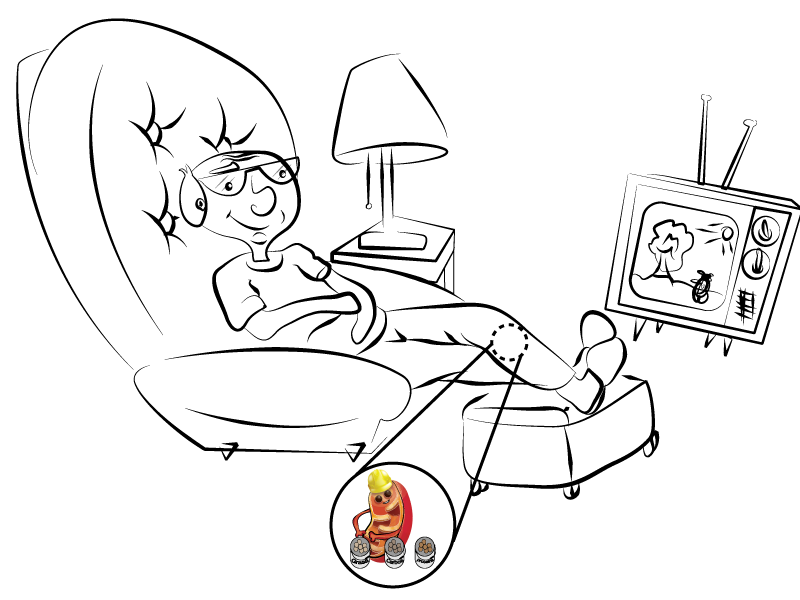
\includegraphics[width=80mm]{./Figures/instauracionFatigaReposo_1_3}} 
\subfigure[Mi metus, sed bibendum ligula efficitur eu.]{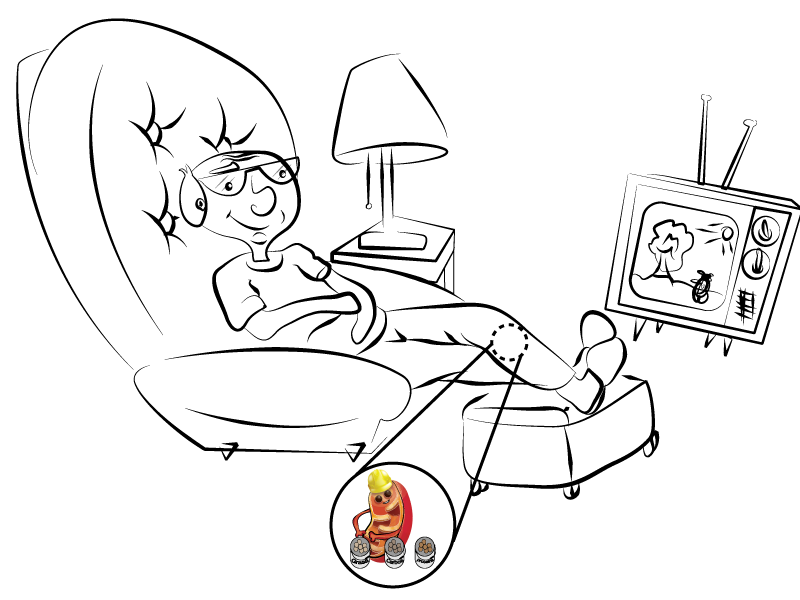
\includegraphics[width=80mm]{./Figures/instauracionFatigaReposo_1_3}}
\subfigure[Mi metus, sed bibendum ligula efficitur eu.]{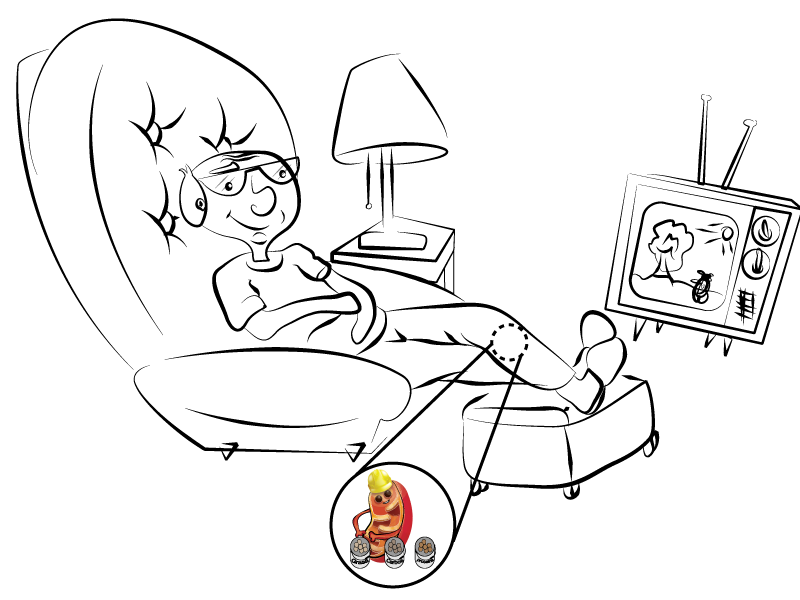
\includegraphics[width=160mm]{./Figures/instauracionFatigaReposo_1_3}}
\caption{Lorem ipsum dolor sit amet, consectetur adipiscing elit. Aliquam sit amet lobortis turpis. Praesent auctor mi metus.  } \label{fig:instauracionFatigaReposo}
\end{figure}





\newpage
%%=====================================================
